% ==== Machine Learning =============================================================================
\chapter{Machine Learning}
\section{Introduction to Machine Learning}

% ---- 5.1.1 What is Machine Learning? -----------------------------------------------------------
\subsection{What is Machine Learning?}

\begin{tcbitemize}[ skin=sectionraster ]
    \tcbitem[title=What is Machine Learning?, raster multicolumn=3]
    Machine learning (ML) is the study of algorithms that improve their performance at a task through experience\textsuperscript{\cite[][pp.~8--10]{iiiCourseMachineLearning}}.
    Rather than being explicitly programmed with rules, an ML algorithm learns patterns from data.
    A learning algorithm receives training examples and produces a model (also called a hypothesis) that can make predictions on previously unseen inputs.

    \tcbitem[title=ML Components, raster multicolumn=3]
    \begin{tblr}{|Q[c,m]|X|X|}
        \hline
        \textbf{Component}   & \textbf{Description}                          & \textbf{Example}                              \\
        \hline
        Training data        & Labeled or unlabeled examples                 & 10\,000 images with ``cat''/``dog'' labels     \\
        \hline
        Model / Hypothesis   & Function learned from data                    & $f(\mathbf{x}) = \mathbf{w}^\top\mathbf{x}+b$ \\
        \hline
        Loss function        & Measures prediction error                     & $\ell(y,\hat{y}) = (y-\hat{y})^2$             \\
        \hline
        Optimization         & Finds parameters minimizing the loss          & Gradient descent, normal equation              \\
        \hline
    \end{tblr}

    \tcbitem[title=The Learning Pipeline, raster multicolumn=6]
    Every ML project follows a common pipeline: collect and prepare data, select features, choose and train a model, evaluate it on held-out data, and deploy it.
    The \emph{inductive bias} of a learning algorithm determines which solutions it prefers when data alone is insufficient to uniquely determine a model\textsuperscript{\cite[][p.~15]{iiiCourseMachineLearning}}.
    \tcblower
    \begin{center}
    \begin{tikzpicture}[
        node distance=0.3cm,
        every node/.style={draw, rounded corners, minimum height=0.7cm, minimum width=1.6cm, font=\sffamily\footnotesize, align=center},
        arr/.style={-{Stealth[length=2mm]}, thick}
    ]
        \node (data) {Raw\\Data};
        \node (prep) [right=of data] {Pre-\\processing};
        \node (feat) [right=of prep] {Feature\\Engineering};
        \node (train) [right=of feat] {Model\\Training};
        \node (eval) [right=of train] {Evaluation};
        \node (deploy) [right=of eval] {Deployment};
        \draw[arr] (data) -- (prep);
        \draw[arr] (prep) -- (feat);
        \draw[arr] (feat) -- (train);
        \draw[arr] (train) -- (eval);
        \draw[arr] (eval) -- (deploy);
    \end{tikzpicture}
    \end{center}
\end{tcbitemize}

% ---- 5.1.2 Supervised & Unsupervised Learning --------------------------------------------------
\subsection{Supervised \& Unsupervised Learning}

\begin{tcbitemize}[ skin=sectionraster ]
    \tcbitem[title=Supervised Learning, raster multicolumn=3]
    In supervised learning, the training data consists of input--output pairs $(\mathbf{x}_n, y_n)$\textsuperscript{\cite[][pp.~8--12]{iiiCourseMachineLearning}}.
    The algorithm learns a mapping $f: \mathbf{x} \mapsto y$ that generalizes to unseen inputs.
    The two main supervised tasks are \textbf{classification} (discrete $y$) and \textbf{regression} (continuous $y$).
    \tcblower
    \begin{itemize}
        \item Labels provided during training
        \item Optimizes a loss w.r.t.\ known outputs
        \item Examples: logistic regression, SVM, random forest, neural networks
    \end{itemize}

    \tcbitem[title=Unsupervised Learning, raster multicolumn=3]
    In unsupervised learning, only the inputs $\mathbf{x}_n$ are given---there are no labels\textsuperscript{\cite[][p.~166]{iiiCourseMachineLearning}}.
    The algorithm must discover hidden structure such as clusters, latent factors, or density estimates.
    \tcblower
    \begin{itemize}
        \item No labels; discovers structure from data alone
        \item Optimizes cohesion/separation or likelihood
        \item Examples: K-means, DBSCAN, PCA, autoencoders
    \end{itemize}

    \tcbitem[title=Classification vs.\ Clustering, raster multicolumn=6]
    Classification and clustering both produce groups, but they differ fundamentally in their inputs and objectives\textsuperscript{\cite[][pp.~323--324]{hurbansGrokkingArtificialIntelligence2020}}.
    \tcblower
    \begin{tblr}{|Q[c,m]|X|X|}
        \hline
        \textbf{Aspect}     & \textbf{Classification}                       & \textbf{Clustering}                                  \\
        \hline
        Learning type       & Supervised (with labels)                      & Unsupervised (without labels)                        \\
        \hline
        Main question       & ``Which known class does $x$ belong to?''     & ``What natural groups exist in the data?''           \\
        \hline
        Output              & Predefined class labels                       & Newly discovered clusters                            \\
        \hline
        Typical algorithms  & Logistic regression, SVM, random forest, k-NN & K-means, DBSCAN, hierarchical clustering, GMM        \\
        \hline
        Evaluation          & Accuracy, F1, ROC-AUC                         & Silhouette, within-cluster variance, domain judgment \\
        \hline
    \end{tblr}
\end{tcbitemize}

% ---- 5.1.3 Regression & Classification ---------------------------------------------------------
\subsection{Regression \& Classification}

\begin{tcbitemize}[ skin=sectionraster ]
    \tcbitem[title=Regression, raster multicolumn=3]
    Regression predicts a continuous real-valued output.
    The model minimizes expected loss over the data distribution\textsuperscript{\cite[][pp.~8--9]{iiiCourseMachineLearning}}.
    Typical loss functions include squared error and absolute error.
    \tcblower
    \begin{equation}
        \hat{\varepsilon} = \frac{1}{N}\sum_{n=1}^{N}(y_n - f(\mathbf{x}_n))^2
    \end{equation}
    Evaluation: MSE, RMSE, MAE, $R^2$.

    \tcbitem[title=Classification, raster multicolumn=3]
    Classification predicts a discrete class label.
    The model learns a decision boundary separating the classes\textsuperscript{\cite[][pp.~10--12]{iiiCourseMachineLearning}}.
    The ideal loss is zero/one, but smooth surrogates (logistic loss, hinge loss) are used in practice.
    \tcblower
    \begin{equation}
        \ell^{(0/1)}(y, \hat{y}) = \begin{cases} 0 & \text{if } y = \hat{y} \\ 1 & \text{otherwise} \end{cases}
    \end{equation}
    Evaluation: Accuracy, Precision, Recall, F1, ROC-AUC.
\end{tcbitemize}

% ---- 5.1.4 Reinforcement Learning (Overview) ---------------------------------------------------
\subsection{Reinforcement Learning}

\begin{tcbitemize}[ skin=sectionraster ]
    \tcbitem[title=Reinforcement Learning Overview, raster multicolumn=3]
    In reinforcement learning (RL), an agent learns by interacting with an environment: it observes states, takes actions, and receives rewards\textsuperscript{\cite[][pp.~323--345]{hurbansGrokkingArtificialIntelligence2020}}.
    The goal is to learn a policy that maximizes cumulative reward over time.
    Unlike supervised learning, correct actions are not given---the agent must discover them through trial and error.
    See Chapter~7 for a detailed treatment.

    \tcbitem[title=Agent--Environment Loop, raster multicolumn=3]
    \begin{center}
    \begin{tikzpicture}[
        node distance=1.8cm,
        every node/.style={draw, rounded corners, minimum height=0.8cm, minimum width=2cm, font=\sffamily\footnotesize, align=center},
        arr/.style={-{Stealth[length=2mm]}, thick}
    ]
        \node (agent) {Agent};
        \node (env) [right=of agent] {Environment};
        \draw[arr] ([yshift=3mm]agent.east) -- node[above, draw=none, minimum height=0, minimum width=0] {\footnotesize action $a_t$} ([yshift=3mm]env.west);
        \draw[arr] ([yshift=-3mm]env.west) -- node[below, draw=none, minimum height=0, minimum width=0] {\footnotesize state $s_{t+1}$, reward $r_{t+1}$} ([yshift=-3mm]agent.east);
    \end{tikzpicture}
    \end{center}
\end{tcbitemize}

% ---- 5.1.5 Model Evaluation & Overfitting ------------------------------------------------------
\subsection{Model Evaluation \& Overfitting}

\begin{tcbitemize}[ skin=sectionraster ]
    \tcbitem[title=Bias--Variance Trade-off, raster multicolumn=6]
    A model's prediction error decomposes into three components: bias (systematic error from simplifying assumptions), variance (sensitivity to training data fluctuations), and irreducible noise\textsuperscript{\cite[][pp.~14--25]{iiiCourseMachineLearning}}.
    \emph{Underfitting} (high bias) occurs when the model is too simple; \emph{overfitting} (high variance) occurs when the model memorizes noise in the training data.
    \tcblower
    \begin{equation}
        \text{Error} = \text{Bias}^2 + \text{Variance} + \text{Irreducible Noise}
    \end{equation}

    \tcbitem[title=Train/Validation/Test Split, raster multicolumn=3]
    To estimate generalization performance, data is split into three disjoint sets\textsuperscript{\cite[][pp.~18--20]{iiiCourseMachineLearning}}:
    \begin{itemize}
        \item \textbf{Training set:} used to fit model parameters
        \item \textbf{Validation set:} used to tune hyperparameters and select models
        \item \textbf{Test set:} held out until the very end to estimate true performance
    \end{itemize}
    A common split ratio is 60/20/20 or 70/15/15.

    \tcbitem[title=Cross-Validation, raster multicolumn=3]
    $k$-fold cross-validation partitions the data into $k$ equal folds.
    The model is trained $k$ times, each time using a different fold as validation and the remaining $k{-}1$ folds for training\textsuperscript{\cite[][pp.~20--22]{iiiCourseMachineLearning}}.
    \tcblower
    \begin{equation}
        \text{CV}(k) = \frac{1}{k}\sum_{i=1}^{k} \text{Error}_i
    \end{equation}
    Typical choice: $k = 5$ or $k = 10$.
\end{tcbitemize}
\section{Clustering}

% ---- 5.2.1 Introduction to Clustering ---------------------------------------------------------
\subsection{Introduction to Clustering}

\begin{tcbitemize}[ skin=sectionraster ]
    \tcbitem[title=What is Clustering?, raster multicolumn=3]
    Clustering is unsupervised learning that partitions data into groups (clusters) such that objects within a cluster are more similar to each other than to objects in other clusters\textsuperscript{\cite[][p.166]{iiiCourseMachineLearning}}. Unlike classification, there are no predefined class labels; the algorithm discovers structure from the data alone.

    \tcbitem[title=Clustering Families, raster multicolumn=3]
    \begin{tblr}{|Q[c,m]|X|X|}
        \hline
        \textbf{Family}      & \textbf{Representative Algorithm} & \textbf{Key Idea}                          \\
        \hline
        Partitioning         & K-Means                           & Minimize within-cluster sum of squares     \\
        \hline
        Hierarchical         & Agglomerative / Divisive          & Build nested cluster tree (dendrogram)     \\
        \hline
        Density-based        & DBSCAN                            & Clusters as dense, connected regions       \\
        \hline
        Model-based          & GMM / EM                          & Mixture of Gaussian distributions          \\
        \hline
    \end{tblr}

    \tcbitem[title=Evaluating Cluster Quality, raster multicolumn=6]
    Because there are no labels, clustering quality must be assessed by internal criteria\textsuperscript{\cite[][pp.~443--445]{hanDataMiningConcepts2012}}. The silhouette coefficient $s(i)$ combines cohesion (average intra-cluster distance $a(i)$) and separation (average distance to the nearest other cluster $b(i)$) into a single score in $[-1, 1]$.
    \tcblower
    \begin{equation}
        s(i) = \frac{b(i) - a(i)}{\max\{a(i),\, b(i)\}}, \qquad s(i) \in [-1,\, 1]
    \end{equation}
\end{tcbitemize}

% ---- 5.2.2 K-Means -----------------------------------------------------------------------------
\subsection{K-Means}

\begin{tcbitemize}[ skin=sectionraster ]
    \tcbitem[title=K-Means Objective, raster multicolumn=3]
    K-means partitions $N$ data points into $K$ clusters by minimizing the within-cluster sum of squared distances to the cluster centroid\textsuperscript{\cite[][p.166]{iiiCourseMachineLearning}}. The algorithm alternates between assigning each point to its nearest centroid and recomputing each centroid as the mean of its assigned points.
    \tcblower
    \begin{equation}
        \mathcal{L}(\mathbf{z}, \boldsymbol{\mu}) = \sum_{k=1}^{K} \sum_{n:\, z_n = k} \|\mathbf{x}_n - \boldsymbol{\mu}_k\|^2
    \end{equation}

    \tcbitem[title=K-Means Algorithm, raster multicolumn=3]
    K-means is guaranteed to converge (the objective decreases monotonically at each step) but only to a local optimum\textsuperscript{\cite[][pp.~166--168]{iiiCourseMachineLearning}}. Initialization therefore strongly affects the solution quality.
    \tcblower
    \begin{enumerate}
        \item Initialize $K$ cluster centroids $\boldsymbol{\mu}_1, \ldots, \boldsymbol{\mu}_K$
        \item \textbf{Assign:} $z_n \leftarrow \arg\min_k \|\mathbf{x}_n - \boldsymbol{\mu}_k\|^2$ for every point $n$
        \item \textbf{Update:} $\boldsymbol{\mu}_k \leftarrow \dfrac{1}{|C_k|}\displaystyle\sum_{n \in C_k} \mathbf{x}_n$ for every cluster $k$
        \item Repeat steps 2--3 until convergence (no assignment changes)
    \end{enumerate}

    \tcbitem[title=K-Means++ Initialization, raster multicolumn=3]
    K-means++ improves the standard random initialization by spreading the initial centroids across the data\textsuperscript{\cite[][pp.~168--169]{iiiCourseMachineLearning}}. The first centroid is chosen uniformly at random; each subsequent centroid is chosen with probability proportional to $D(\mathbf{x})^2$, the squared distance to the nearest existing centroid. This yields the approximation guarantee below.
    \tcblower
    \begin{equation}
        \mathbb{E}\bigl[\hat{\mathcal{L}}\bigr] \leq 8(\log K + 2)\,\mathcal{L}^{(\mathrm{opt})}
    \end{equation}

    \tcbitem[title={Choosing K: Elbow Method and Information Criteria}, raster multicolumn=3]
    There is no single best method for choosing $K$\textsuperscript{\cite[][p.169]{iiiCourseMachineLearning}}. The elbow method plots the within-cluster sum of squares (WCSS) against $K$ and selects the value at which improvement begins to plateau. Information criteria penalize model complexity explicitly.
    \tcblower
    \begin{equation}
        \text{BIC:}\; \arg\min_K \hat{\mathcal{L}}_K + K\log D
        \qquad
        \text{AIC:}\; \arg\min_K \hat{\mathcal{L}}_K + 2KD
    \end{equation}
\end{tcbitemize}

% ---- 5.2.3 Expectation Maximization ------------------------------------------------------------
\subsection{Expectation Maximization}

\begin{tcbitemize}[ skin=sectionraster ]
    \tcbitem[title=Gaussian Mixture Models (GMM), raster multicolumn=3]
    A Gaussian Mixture Model assumes data are generated from $K$ Gaussian components with mixing weights $\theta_k$, means $\boldsymbol{\mu}_k$, and covariances $\boldsymbol{\Sigma}_k$\textsuperscript{\cite[][p.175]{iiiCourseMachineLearning}}. Unlike K-means (hard, binary assignments), GMM fitting via EM produces \emph{soft} (probabilistic) memberships: each point belongs to every cluster to some degree.
    \tcblower
    \begin{equation}
        p(\mathbf{x}) = \sum_{k=1}^{K} \theta_k \,\mathcal{N}(\mathbf{x} \mid \boldsymbol{\mu}_k, \boldsymbol{\Sigma}_k), \qquad \sum_{k=1}^{K}\theta_k = 1
    \end{equation}

    \tcbitem[title={E-Step: Computing Responsibilities}, raster multicolumn=3]
    In the Expectation step, the current parameters are held fixed and the posterior probability (responsibility) that component $k$ generated point $\mathbf{x}_n$ is computed\textsuperscript{\cite[][pp.~175--177]{iiiCourseMachineLearning}}. These soft assignments $z_{n,k}$ replace the hard assignments $z_n$ of K-means.
    \tcblower
    \begin{equation}
        z_{n,k} = \frac{\theta_k \,\mathcal{N}(\mathbf{x}_n \mid \boldsymbol{\mu}_k, \boldsymbol{\Sigma}_k)}
                       {\displaystyle\sum_{j=1}^{K} \theta_j \,\mathcal{N}(\mathbf{x}_n \mid \boldsymbol{\mu}_j, \boldsymbol{\Sigma}_j)}
    \end{equation}

    \tcbitem[title={M-Step: Re-estimating Parameters}, raster multicolumn=6]
    In the Maximization step, the responsibilities are held fixed and the model parameters are updated to maximize the expected log-likelihood\textsuperscript{\cite[][pp.~177--178]{iiiCourseMachineLearning}}. Each iteration of EM is guaranteed to increase (or maintain) the log-likelihood.
    \tcblower
    \begin{equation}
        \theta_k = \frac{1}{N}\sum_{n=1}^{N} z_{n,k}, \qquad
        \boldsymbol{\mu}_k = \frac{\sum_n z_{n,k}\,\mathbf{x}_n}{\sum_n z_{n,k}}, \qquad
        \boldsymbol{\Sigma}_k = \frac{\sum_n z_{n,k}(\mathbf{x}_n - \boldsymbol{\mu}_k)(\mathbf{x}_n - \boldsymbol{\mu}_k)^\top}{\sum_n z_{n,k}}
    \end{equation}

    \tcbitem[title=EM as a Generalization of K-Means, raster multicolumn=6]
    K-means is a special case of EM\textsuperscript{\cite[][p.180]{iiiCourseMachineLearning}}. When all GMM covariances are fixed to $\sigma^2 \mathbf{I}$ and $\sigma \to 0$, the soft responsibilities $z_{n,k}$ collapse to hard indicator assignments and the EM update reduces exactly to the K-means update. EM thus trades the assumption of spherical, equal-size clusters for the ability to model elliptical clusters of varying shapes and sizes.
    \tcblower
    \begin{tblr}{|X|X|X|}
        \hline
                                & \textbf{K-Means}          & \textbf{EM / GMM}                    \\
        \hline
        Assignments             & Hard (binary)             & Soft (probabilistic)                 \\
        \hline
        Cluster shape           & Spherical, equal-size     & Elliptical, varying size             \\
        \hline
        Parameters learned      & Centroids $\boldsymbol{\mu}_k$ & $\boldsymbol{\mu}_k$, $\boldsymbol{\Sigma}_k$, $\theta_k$ \\
        \hline
        Convergence guarantee   & Local optimum of WCSS     & Monotone increase of log-likelihood  \\
        \hline
    \end{tblr}
\end{tcbitemize}

% ---- 5.2.4 DBSCAN ------------------------------------------------------------------------------
\subsection{DBSCAN}

\begin{tcbitemize}[ skin=sectionraster, halign lower=center ]
    \tcbitem[title=Density-Based Clustering Concept, raster multicolumn=3]
    DBSCAN (Density-Based Spatial Clustering of Applications with Noise) identifies clusters as dense regions of points separated by sparser regions\textsuperscript{\cite[][p.471]{hanDataMiningConcepts2012}}. It requires two parameters: the neighborhood radius $\varepsilon$ and the minimum point count MinPts. Crucially, DBSCAN requires no preset number of clusters $K$ and naturally labels low-density points as noise (outliers).

    \tcbitem[title={Core, Border, and Noise Points}, raster multicolumn=3]
    Every point in DBSCAN is classified as exactly one of three types based on the density of its $\varepsilon$-neighborhood $N_\varepsilon(p) = \{q \mid d(p,q) \leq \varepsilon\}$\textsuperscript{\cite[][pp.~472--474]{hanDataMiningConcepts2012}}. A cluster is the maximal set of density-connected core and border points.
    \tcblower
    \begin{tblr}{|Q[c,m]|X|}
        \hline
        \textbf{Point type} & \textbf{Definition}                                                          \\
        \hline
        Core point          & $|N_\varepsilon(p)| \geq \text{MinPts}$ — enough neighbors to start a cluster \\
        \hline
        Border point        & $|N_\varepsilon(p)| < \text{MinPts}$ but within $\varepsilon$ of a core point  \\
        \hline
        Noise point         & Neither core nor border — an outlier                                         \\
        \hline
    \end{tblr}

    \tcbitem[title=DBSCAN Point Types Illustrated, raster multicolumn=6]
    With MinPts $= 4$ and radius $\varepsilon$, core points have dense neighborhoods, border points are nearby but sparse, and noise points are isolated\textsuperscript{\cite[][p.473]{hanDataMiningConcepts2012}}.
    \tcblower
    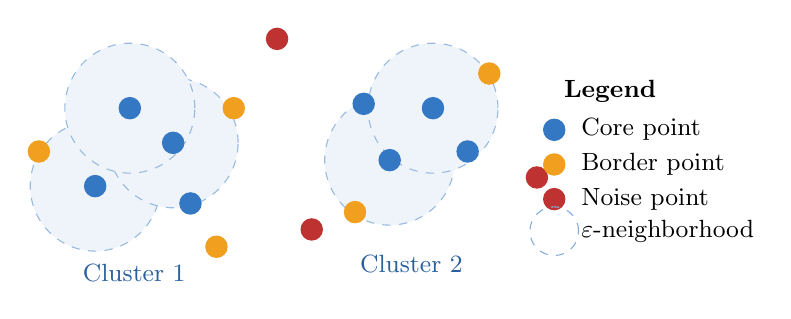
\begin{tikzpicture}[scale=1.1]
        % -- colour definitions --------------------------------------------------
        \definecolor{corecolor}{RGB}{52,120,196}
        \definecolor{bordercolor}{RGB}{240,160,30}
        \definecolor{noisecolor}{RGB}{190,50,50}

        % -- epsilon circles around core points (light fill) ---------------------
        \foreach \cx/\cy in {0/0, 0.9/0.5, 0.4/0.9} {
            \draw[dashed, corecolor!50, fill=corecolor!8, thin]
                (\cx,\cy) circle (0.75);
        }

        % -- cluster 1: core points ----------------------------------------------
        \foreach \px/\py in {0/0, 0.9/0.5, 0.4/0.9, 1.1/-0.2} {
            \filldraw[corecolor] (\px,\py) circle (3.5pt);
        }

        % -- cluster 1: border points -------------------------------------------
        \foreach \px/\py in {-0.65/0.4, 1.6/0.9, 1.4/-0.7} {
            \filldraw[bordercolor] (\px,\py) circle (3.5pt);
        }

        % -- cluster 2: two core points + border --------------------------------
        \foreach \cx/\cy in {3.4/0.3, 3.9/0.9} {
            \draw[dashed, corecolor!50, fill=corecolor!8, thin]
                (\cx,\cy) circle (0.75);
        }
        \foreach \px/\py in {3.4/0.3, 3.9/0.9, 3.1/0.95, 4.3/0.4} {
            \filldraw[corecolor] (\px,\py) circle (3.5pt);
        }
        \foreach \px/\py in {3.0/-0.3, 4.55/1.3} {
            \filldraw[bordercolor] (\px,\py) circle (3.5pt);
        }

        % -- noise points --------------------------------------------------------
        \foreach \px/\py in {2.1/1.7, 2.5/-0.5, 5.1/0.1} {
            \filldraw[noisecolor] (\px,\py) circle (3.5pt);
        }

        % -- legend --------------------------------------------------------------
        \node[right] at (5.3, 1.1)  {\small\textbf{Legend}};
        \filldraw[corecolor]   (5.3, 0.65) circle (3.5pt);
        \node[right] at (5.5, 0.65) {\small Core point};
        \filldraw[bordercolor] (5.3, 0.25) circle (3.5pt);
        \node[right] at (5.5, 0.25) {\small Border point};
        \filldraw[noisecolor]  (5.3,-0.15) circle (3.5pt);
        \node[right] at (5.5,-0.15) {\small Noise point};
        \draw[dashed, corecolor!60, thin] (5.3,-0.52) circle (8pt);
        \node[right] at (5.5,-0.52) {\small $\varepsilon$-neighborhood};

        % -- cluster labels ------------------------------------------------------
        \node[corecolor!80!black] at (0.45,-1.0) {\small Cluster 1};
        \node[corecolor!80!black] at (3.65,-0.9) {\small Cluster 2};
    \end{tikzpicture}

    \tcbitem[title=DBSCAN Algorithm, raster multicolumn=6]
    DBSCAN visits each unvisited point, expands a new cluster if a core point is found, and marks isolated points as noise\textsuperscript{\cite[][pp.~474--477]{hanDataMiningConcepts2012}}. With a spatial index (e.g.\ R-tree), complexity is $O(n \log n)$; without indexing it degrades to $O(n^2)$.
    \tcblower
    \begin{enumerate}
        \item For each unvisited point $p$: compute $N_\varepsilon(p)$
        \item If $|N_\varepsilon(p)| \geq \text{MinPts}$: mark $p$ as a core point, start a new cluster $C$
        \item Expand $C$: add all points density-reachable from $p$ (recursively include core points found)
        \item If $|N_\varepsilon(p)| < \text{MinPts}$: mark $p$ as noise (may later become a border point of another cluster)
        \item Repeat until all points are visited
    \end{enumerate}
\end{tcbitemize}

% ---- 5.2.5 Hierarchical Clustering -------------------------------------------------------------
\subsection{Hierarchical Clustering}

\begin{tcbitemize}[ skin=sectionraster, halign lower=center ]
    \tcbitem[title=Agglomerative Hierarchical Clustering, raster multicolumn=3]
    Hierarchical clustering builds a tree-like decomposition of data called a dendrogram\textsuperscript{\cite[][p.457]{hanDataMiningConcepts2012}}. The agglomerative (bottom-up) approach starts with each data point as its own singleton cluster and iteratively merges the two closest clusters until only one remains. The number of clusters $K$ need not be specified in advance: it is determined by cutting the dendrogram at the desired height.
    \tcblower
    \begin{enumerate}
        \item Start: assign each of the $n$ points to its own cluster
        \item Compute the $n \times n$ pairwise distance matrix
        \item Merge the two clusters with the smallest inter-cluster distance
        \item Update the distance matrix (recompute distances to the merged cluster)
        \item Repeat steps 3--4 until one cluster remains
        \item Cut the dendrogram at the desired level to obtain $K$ clusters
    \end{enumerate}

    \tcbitem[title=Linkage Criteria, raster multicolumn=3]
    The choice of linkage criterion defines how the distance between two clusters $C_i$ and $C_j$ is measured and strongly affects the shape of the resulting clusters\textsuperscript{\cite[][pp.~460--463]{hanDataMiningConcepts2012}}.
    \tcblower
    \begin{tblr}{|Q[l,m,wd=2.6cm]|X|X|}
        \hline
        \textbf{Linkage}  & \textbf{Formula}                                                                                              & \textbf{Effect}                       \\
        \hline
        Single            & $\min_{p \in C_i,\, q \in C_j} d(p,q)$                                                                       & Chain-shaped, elongated clusters      \\
        \hline
        Complete          & $\max_{p \in C_i,\, q \in C_j} d(p,q)$                                                                       & Compact, spherical clusters           \\
        \hline
        Average (UPGMA)   & $\dfrac{1}{|C_i||C_j|}\displaystyle\sum_{p \in C_i}\sum_{q \in C_j} d(p,q)$                                  & Compromise between single and complete \\
        \hline
        Ward's method     & Merges pair minimizing increase in total within-cluster variance                                              & Compact, equal-size clusters          \\
        \hline
    \end{tblr}

    \tcbitem[title=Reading a Dendrogram, raster multicolumn=6]
    The height of each merge in the dendrogram encodes the inter-cluster distance at which two groups were joined\textsuperscript{\cite[][pp.~457--467]{hanDataMiningConcepts2012}}. A horizontal cut at height $h$ produces the clustering at that granularity: every connected subtree below the cut is one cluster. Large vertical gaps between merges indicate a natural number of clusters.
    \tcblower
    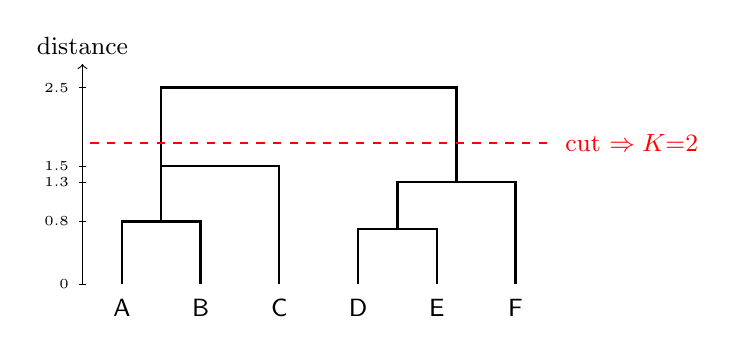
\begin{tikzpicture}[scale=1.0]
        % -- leaf labels (6 points: A..F) ----------------------------------------
        \foreach \lbl/\x in {A/0, B/1, C/2, D/3, E/4, F/5} {
            \node[font=\small\sffamily] at (\x, -0.3) {\lbl};
        }

        % -- merge 1: A+B at height 0.8 ------------------------------------------
        \draw[thick] (0, 0) -- (0, 0.8) -- (1, 0.8) -- (1, 0);

        % -- merge 2: D+E at height 0.7 ------------------------------------------
        \draw[thick] (3, 0) -- (3, 0.7) -- (4, 0.7) -- (4, 0);

        % -- merge 3: (D+E)+F at height 1.3 --------------------------------------
        \draw[thick] (3.5, 0.7) -- (3.5, 1.3) -- (5, 1.3) -- (5, 0);

        % -- merge 4: (A+B)+C at height 1.5 --------------------------------------
        \draw[thick] (0.5, 0.8) -- (0.5, 1.5) -- (2, 1.5) -- (2, 0);

        % -- merge 5: cluster{A,B,C} + cluster{D,E,F} at height 2.5 -------------
        \draw[thick] (0.5, 1.5) -- (0.5, 2.5) -- (4.25, 2.5) -- (4.25, 1.3);

        % -- cut line at height 1.8 ----------------------------------------------
        \draw[red, dashed, thick] (-0.4, 1.8) -- (5.5, 1.8)
            node[right, font=\small, text=red] {cut $\Rightarrow K{=}2$};

        % -- y-axis label --------------------------------------------------------
        \draw[->] (-0.5, 0) -- (-0.5, 2.8) node[above, font=\small] {distance};
        \foreach \y/\lbl in {0/0, 0.8/0.8, 1.3/1.3, 1.5/1.5, 2.5/2.5} {
            \draw (-0.55,\y) -- (-0.45,\y);
            \node[left, font=\tiny] at (-0.55,\y) {\lbl};
        }
    \end{tikzpicture}
\end{tcbitemize}
\section{Regression}

% ---- 5.3.1 Linear & Non-linear Regression -------------------------------------------------------
\subsection{Linear \& Non-linear Regression}

\begin{tcbitemize}[ skin=sectionraster ]
    \tcbitem[title={Linear Regression and the Normal Equation}, raster multicolumn=3]
    Linear regression fits a linear function $\hat{y} = \mathbf{w}^\top \mathbf{x} + b$ by minimizing the sum of squared residuals (Ordinary Least Squares)\textsuperscript{\cite[][pp.~86--90]{iiiCourseMachineLearning}}. When the design matrix $\mathbf{X}$ has full column rank, the unique minimizer is given in closed form by the normal equation.
    \tcblower
    \begin{equation}
        \underbrace{\min_{\mathbf{w}} \|\mathbf{X}\mathbf{w} - \mathbf{y}\|^2}_{\text{OLS objective}}
        \quad\Longrightarrow\quad
        \hat{\mathbf{w}} = (\mathbf{X}^\top\mathbf{X})^{-1}\mathbf{X}^\top\mathbf{y}
    \end{equation}

    \tcbitem[title={Polynomial and Non-linear Regression}, raster multicolumn=3]
    Non-linear regression extends the linear model by mapping inputs through basis functions $\phi_j(\mathbf{x})$, e.g.\ polynomial features $[1, x, x^2, \ldots, x^d]$\textsuperscript{\cite[][pp.~90--97]{iiiCourseMachineLearning}}. The model remains \emph{linear in the parameters} $\mathbf{w}$, so the normal equation still applies. High-degree polynomials can overfit (high variance), motivating regularization.
    \tcblower
    \begin{equation}
        \hat{y} = \sum_{j=0}^{d} w_j\, x^j = \mathbf{w}^\top \boldsymbol{\phi}(x),
        \qquad \boldsymbol{\phi}(x) = [1,\, x,\, x^2,\, \ldots,\, x^d]^\top
    \end{equation}
\end{tcbitemize}

% ---- 5.3.2 Logistic Regression ------------------------------------------------------------------
\subsection{Logistic Regression}

\begin{tcbitemize}[ skin=sectionraster, halign lower=center ]
    \tcbitem[title={Logistic Regression as a Classification Model}, raster multicolumn=3]
    Despite its name, logistic regression is a \emph{classification} method. It models the probability of class membership by mapping a linear combination of features through the logistic (sigmoid) function $\sigma$, squashing any real value into the interval $[0, 1]$\textsuperscript{\cite[][pp.~89--90]{iiiCourseMachineLearning}}. Training maximizes the likelihood (no closed-form solution; gradient descent is used).
    \tcblower
    \begin{equation}
        P(y = 1 \mid \mathbf{x}) = \sigma\!\left(\mathbf{w}^\top \mathbf{x} + b\right) = \frac{1}{1 + \exp\!\left[-\!\left(\mathbf{w}^\top \mathbf{x} + b\right)\right]}
    \end{equation}

    \tcbitem[title={The Sigmoid Curve and Log-Odds}, raster multicolumn=3]
    The sigmoid function produces the characteristic S-shaped curve shown below\textsuperscript{\cite[][p.89]{iiiCourseMachineLearning}}. In log-odds (logit) form, the model is linear: $\log\frac{P(y=1|\mathbf{x})}{1-P(y=1|\mathbf{x})} = \mathbf{w}^\top\mathbf{x} + b$. The logistic loss $\ell^{(\log)}(y,\hat{y}) = \log(1 + \exp[-y\hat{y}])$ is a smooth, convex surrogate for the 0/1 loss.
    \tcblower
    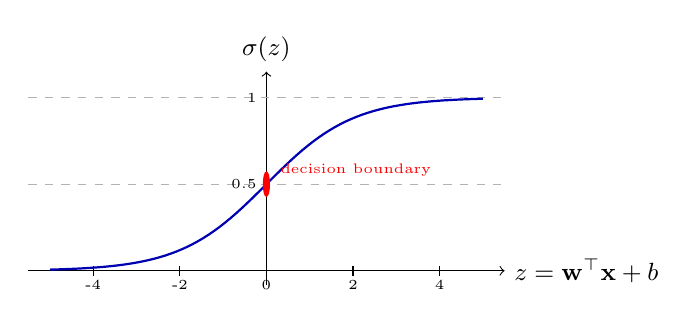
\begin{tikzpicture}[scale=1.0]
        \begin{scope}[xscale=0.55, yscale=2.2]
            % axes
            \draw[->] (-5.5,0) -- (5.5,0) node[right, font=\small] {$z = \mathbf{w}^\top\mathbf{x}+b$};
            \draw[->] (0,-0.08) -- (0,1.15) node[above, font=\small] {$\sigma(z)$};
            % dashed reference lines
            \draw[dashed, gray!60] (-5.5,1) -- (5.5,1);
            \draw[dashed, gray!60] (-5.5,0.5) -- (5.5,0.5);
            % tick marks
            \foreach \x in {-4,-2,0,2,4} {
                \draw (\x,0.03) -- (\x,-0.03);
                \node[below, font=\tiny] at (\x,0) {\x};
            }
            \node[left, font=\tiny] at (0,1)   {$1$};
            \node[left, font=\tiny] at (0,0.5) {$0.5$};
            % sigmoid curve
            \draw[thick, blue!70!black, domain=-5:5, samples=80]
                plot (\x, {1/(1+exp(-\x))});
            % decision boundary marker
            \filldraw[red] (0,0.5) circle (2pt);
            \node[right, font=\tiny, text=red] at (0.1, 0.58) {decision boundary};
        \end{scope}
    \end{tikzpicture}
\end{tcbitemize}

% ---- 5.3.3 Quantile Regression ------------------------------------------------------------------
\subsection{Quantile Regression}

\begin{tcbitemize}[ skin=sectionraster ]
    \tcbitem[title={Quantile Regression and the Pinball Loss}, raster multicolumn=6]
    Quantile regression estimates conditional \emph{quantiles} of the response (e.g.\ the median, or the 10th and 90th percentiles) rather than the conditional mean. It is robust to outliers and makes no assumption of normality or homoscedasticity; fitting multiple quantile levels together yields a full prediction interval. The loss function (pinball loss) applies asymmetric linear penalties.
    \tcblower
    \begin{equation}
        \rho_\tau(u) =
        \begin{cases}
            \tau \cdot u       & u \geq 0 \\
            (\tau - 1)\cdot u  & u < 0
        \end{cases},
        \quad
        \min_{\mathbf{w}} \sum_{n=1}^{N} \rho_\tau\!\left(y_n - \mathbf{w}^\top\mathbf{x}_n\right),
        \quad \tau \in (0,1)
    \end{equation}
\end{tcbitemize}

% ---- 5.3.4 Multivariate Regression --------------------------------------------------------------
\subsection{Multivariate Regression}

\begin{tcbitemize}[ skin=sectionraster ]
    \tcbitem[title={Multiple and Multivariate Regression}, raster multicolumn=6]
    Multiple regression extends linear regression to $D$ input features ($\hat{y} = w_0 + w_1 x_1 + \cdots + w_D x_D$); multivariate regression further allows $K$ response variables simultaneously, with coefficient matrix $\mathbf{W} \in \mathbb{R}^{D \times K}$\textsuperscript{\cite[][pp.~86--97]{iiiCourseMachineLearning}}. The same normal equation applies. As $D$ grows, multicollinearity can destabilize $(\mathbf{X}^\top\mathbf{X})^{-1}$, motivating regularization.
    \tcblower
    \begin{equation}
        \hat{\mathbf{Y}} = \mathbf{X}\mathbf{W},
        \qquad
        \hat{\mathbf{W}} = (\mathbf{X}^\top\mathbf{X})^{-1}\mathbf{X}^\top\mathbf{Y}
        \quad (D \text{ features},\; K \text{ responses})
    \end{equation}
\end{tcbitemize}

% ---- 5.3.5 Lasso & Ridge Regression -------------------------------------------------------------
\subsection{Lasso \& Ridge Regression}

\begin{tcbitemize}[ skin=sectionraster, halign lower=center ]
    \tcbitem[title={Ridge Regression (L2) and Lasso (L1)}, raster multicolumn=3]
    Regularized regression adds a penalty on the weights to prevent overfitting\textsuperscript{\cite[][pp.~91--97]{iiiCourseMachineLearning}}. Ridge (L2) shrinks all coefficients uniformly and has a closed-form solution. Lasso (L1) drives some coefficients \emph{exactly} to zero, performing automatic feature selection; it requires iterative solvers (coordinate descent, ISTA). The hyperparameter $\lambda$ controls the bias-variance trade-off.
    \tcblower
    \begin{equation}
        \underbrace{\min_{\mathbf{w}} \tfrac{1}{2}\|\mathbf{X}\mathbf{w}-\mathbf{y}\|^2 + \tfrac{\lambda}{2}\|\mathbf{w}\|_2^2}_{\text{Ridge: } \hat{\mathbf{w}}=(\mathbf{X}^\top\mathbf{X}+\lambda\mathbf{I})^{-1}\mathbf{X}^\top\mathbf{y}}
        \qquad
        \underbrace{\min_{\mathbf{w}} \tfrac{1}{2}\|\mathbf{X}\mathbf{w}-\mathbf{y}\|^2 + \lambda\|\mathbf{w}\|_1}_{\text{Lasso: no closed form}}
    \end{equation}

    \tcbitem[title={Elastic Net and the Geometry of Sparsity}, raster multicolumn=3]
    Elastic Net combines both penalties ($\lambda_1\|\mathbf{w}\|_1 + \lambda_2\|\mathbf{w}\|_2^2$), inheriting Lasso's sparsity and Ridge's stability under multicollinearity\textsuperscript{\cite[][pp.~91--97]{iiiCourseMachineLearning}}. The geometric picture below explains \emph{why} L1 gives sparse solutions: the OLS contours first touch the L1 diamond at a corner (where a coordinate is zero), whereas L1 ellipsoid contacts are typically at smooth points.
    \tcblower
    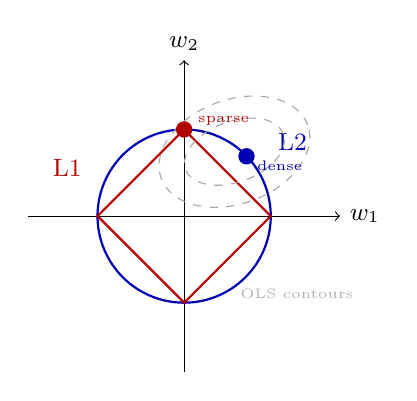
\begin{tikzpicture}[scale=1.1]
        % ---- coordinate axes ----
        \draw[->] (-1.8,0) -- (1.8,0) node[right, font=\small] {$w_1$};
        \draw[->] (0,-1.8) -- (0,1.8) node[above, font=\small] {$w_2$};

        % ---- L2 circle (Ridge constraint) ----
        \draw[thick, blue!70!black] (0,0) circle (1.0);
        \node[blue!70!black, font=\small] at (1.25, 0.85) {L2};

        % ---- L1 diamond (Lasso constraint) ----
        \draw[thick, red!70!black]
            (1.0,0) -- (0,1.0) -- (-1.0,0) -- (0,-1.0) -- cycle;
        \node[red!70!black, font=\small] at (-1.35, 0.55) {L1};

        % ---- OLS contour ellipses (centered off-axis to show contact) ----
        \draw[dashed, gray!70, rotate=20] (0.8,0.5) ellipse (0.6 and 0.35);
        \draw[dashed, gray!70, rotate=20] (0.8,0.5) ellipse (0.9 and 0.6);
        \node[gray!60, font=\tiny] at (1.3,-0.9) {OLS contours};

        % ---- contact points ----
        % L1 corner contact (sparse solution: w1=0 or w2=0)
        \filldraw[red!70!black]  (0, 1.0) circle (2.5pt);
        \node[right, font=\tiny, text=red!70!black] at (0.05, 1.1) {sparse};

        % L2 smooth contact
        \filldraw[blue!70!black] (0.72, 0.69) circle (2.5pt);
        \node[right, font=\tiny, text=blue!70!black] at (0.73, 0.58) {dense};
    \end{tikzpicture}
\end{tcbitemize}

% ===========================================================================================
\section{Support Vector Machines}

% ---- 5.4.1 Introduction to SVMs ----------------------------------------------------------------
\subsection{Introduction to Support Vector Machines}

\begin{tcbitemize}[ skin=sectionraster, halign lower=center ]
    \tcbitem[title={Maximum Margin Hyperplane}, raster multicolumn=6]
    A Support Vector Machine finds the unique hyperplane $\mathbf{w}\cdot\mathbf{x} + b = 0$ that maximizes the geometric margin $\gamma = 2/\|\mathbf{w}\|$ between the two classes\textsuperscript{\cite[][pp.~98--101]{iiiCourseMachineLearning}}. Only the training points closest to the hyperplane — the \emph{support vectors} — determine the solution. The complexity of the learned classifier depends on the number of support vectors, not the dimensionality of the input space.
    \tcblower
    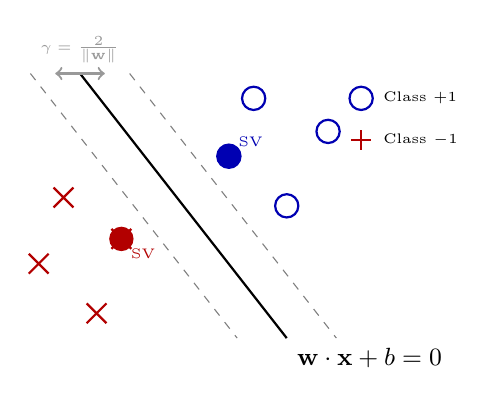
\begin{tikzpicture}[scale=1.05]
        % ---- class A points (circles, top-right) ----
        \foreach \px/\py in {2.8/2.5, 3.5/1.9, 3.1/3.2, 4.0/2.8} {
            \draw[blue!70!black, thick] (\px,\py) circle (4pt);
        }
        % ---- class B points (crosses, bottom-left) ----
        \foreach \px/\py in {0.5/1.2, 1.2/0.6, 0.8/2.0, 1.5/1.5} {
            \draw[red!70!black, thick]
                (\px-0.12,\py-0.12) -- (\px+0.12,\py+0.12)
                (\px+0.12,\py-0.12) -- (\px-0.12,\py+0.12);
        }
        % ---- decision hyperplane ----
        \draw[thick, black] (1.0,3.5) -- (3.5,0.3) node[below right, font=\small] {$\mathbf{w}\cdot\mathbf{x}+b=0$};
        % ---- margin hyperplanes ----
        \draw[dashed, gray]  (0.4,3.5) -- (2.9,0.3);
        \draw[dashed, gray]  (1.6,3.5) -- (4.1,0.3);
        % ---- margin brace ----
        \draw[<->, thick, gray!80] (0.7,3.5) -- (1.3,3.5)
            node[midway, above, font=\tiny] {$\gamma = \frac{2}{\|\mathbf{w}\|}$};
        % ---- support vector highlights ----
        \filldraw[blue!70!black]  (2.8,2.5) circle (4pt);
        \node[above right, font=\tiny, blue!70!black] at (2.8,2.5) {SV};
        \filldraw[red!70!black]   (1.5,1.5) circle (4pt);
        \node[below right, font=\tiny, red!70!black]  at (1.5,1.5) {SV};
        % ---- legend ----
        \draw[blue!70!black, thick] (4.4,3.2) circle (4pt);
        \node[right, font=\tiny] at (4.55,3.2) {Class $+1$};
        \draw[red!70!black, thick]
            (4.28,2.7)--(4.52,2.7) (4.4,2.58)--(4.4,2.82);
        \node[right, font=\tiny] at (4.55,2.7) {Class $-1$};
    \end{tikzpicture}

    \tcbitem[title={Hard-Margin vs.\ Soft-Margin SVM}, raster multicolumn=6]
    Hard-margin SVM requires the data to be linearly separable; soft-margin SVM introduces slack variables $\xi_n \geq 0$ to allow misclassifications, controlled by the cost parameter $C$\textsuperscript{\cite[][pp.~98--101]{iiiCourseMachineLearning}}. Large $C$ penalizes errors heavily (narrow margin, risk of overfitting); small $C$ permits more errors (wider margin, better generalization).
    \tcblower
    \begin{equation}
        \min_{\mathbf{w},b,\boldsymbol{\xi}}\; \frac{1}{2}\|\mathbf{w}\|^2 + C\sum_{n=1}^{N}\xi_n
        \quad\text{s.t.}\quad
        y_n(\mathbf{w}\cdot\mathbf{x}_n + b) \geq 1 - \xi_n,\;\; \xi_n \geq 0 \;\;\forall n
    \end{equation}
\end{tcbitemize}

% ---- 5.4.2 SVM for Classification --------------------------------------------------------------
\subsection{SVM for Classification}

\begin{tcbitemize}[ skin=sectionraster ]
    \tcbitem[title={The Kernel Trick}, raster multicolumn=4]
    For non-linearly separable data, the kernel trick maps inputs into a high-dimensional feature space $\phi(\mathbf{x})$ where a linear separator exists — without ever computing $\phi$ explicitly\textsuperscript{\cite[][pp.~128--140]{iiiCourseMachineLearning}}. The decision function depends only on inner products, which the kernel $K(\mathbf{x}_i,\mathbf{x}_j) = \phi(\mathbf{x}_i)\cdot\phi(\mathbf{x}_j)$ computes directly. SVM training always finds a global optimum (convex QP).
    \tcblower
    \begin{tblr}{|Q[l,m,wd=3.2cm]|X|}
        \hline
        \textbf{Kernel}      & \textbf{Formula}                                                                                      \\
        \hline
        Linear               & $K(\mathbf{x}_i,\mathbf{x}_j) = \mathbf{x}_i\cdot\mathbf{x}_j$                                       \\
        \hline
        Polynomial (degree $h$) & $K(\mathbf{x}_i,\mathbf{x}_j) = (\mathbf{x}_i\cdot\mathbf{x}_j + 1)^h$                            \\
        \hline
        Gaussian RBF         & $K(\mathbf{x}_i,\mathbf{x}_j) = \exp\!\left(-\dfrac{\|\mathbf{x}_i-\mathbf{x}_j\|^2}{2\sigma^2}\right)$ \\
        \hline
        Sigmoid              & $K(\mathbf{x}_i,\mathbf{x}_j) = \tanh(\kappa\,\mathbf{x}_i\cdot\mathbf{x}_j - \delta)$              \\
        \hline
    \end{tblr}

    \tcbitem[title={Multiclass SVMs}, raster multicolumn=2]
    SVMs are inherently binary classifiers. Two standard strategies extend them to $K$ classes\textsuperscript{\cite[][pp.~413--415]{hanDataMiningConcepts2012}}. \emph{One-vs-All} trains $K$ classifiers (class $k$ against all others) and assigns the class with the highest decision score. \emph{One-vs-One} trains $\binom{K}{2}$ binary classifiers and uses majority voting. The decision function for a new point is $d(\mathbf{x}) = \operatorname{sign}\!\left(\sum_{i} y_i \alpha_i K(\mathbf{x}_i, \mathbf{x}) + b_0\right)$.
\end{tcbitemize}

% ---- 5.4.3 SVM for Regression ------------------------------------------------------------------
\subsection{SVM for Regression}

\begin{tcbitemize}[ skin=sectionraster ]
    \tcbitem[title={Support Vector Regression (SVR) and the $\varepsilon$-Tube}, raster multicolumn=6]
    Support Vector Regression applies the maximum-margin principle to regression by defining an $\varepsilon$-insensitive tube around the predicted function\textsuperscript{\cite[][pp.~98--101]{iiiCourseMachineLearning}}. Residuals smaller than $\varepsilon$ incur zero loss; residuals outside the tube are penalized linearly via slack variables $\xi_n, \xi_n^* \geq 0$. Only points outside the tube become support vectors, yielding sparse solutions.
    \tcblower
    \begin{equation}
        \min_{\mathbf{w},b,\boldsymbol{\xi},\boldsymbol{\xi}^*}\; \frac{1}{2}\|\mathbf{w}\|^2 + C\sum_{n=1}^{N}(\xi_n + \xi_n^*)
        \quad\text{s.t.}\quad
        \left|y_n - \mathbf{w}\cdot\mathbf{x}_n - b\right| \leq \varepsilon + \max(\xi_n, \xi_n^*),\;\; \xi_n,\xi_n^* \geq 0
    \end{equation}
\end{tcbitemize}

% ===========================================================================================
\section{Decision Trees \& Ensemble Methods}

% ---- 5.5.1 Introduction to Decision Trees ------------------------------------------------------
\subsection{Introduction to Decision Trees}

\begin{tcbitemize}[ skin=sectionraster, halign lower=center ]
    \tcbitem[title={Decision Trees: Structure and Construction}, raster multicolumn=6]
    A decision tree partitions the feature space recursively: each internal node applies a test on one feature, each branch follows an outcome, and each leaf assigns a prediction\textsuperscript{\cite[][pp.~8--20]{iiiCourseMachineLearning}}. The tree is built greedily (ID3, C4.5, CART) by choosing at each step the feature split that maximizes a purity criterion. Decision trees are highly interpretable but unstable — small data changes can produce very different trees.
    \tcblower
    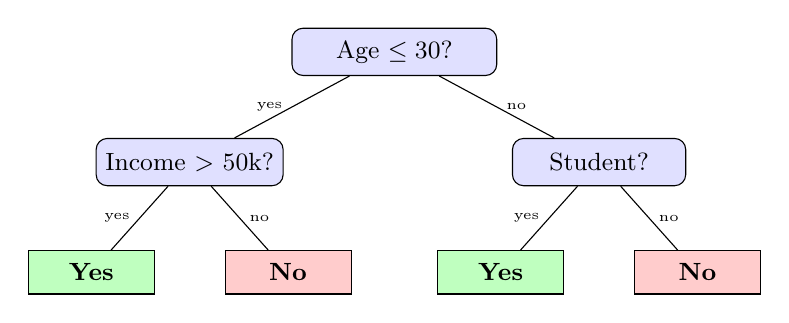
\begin{tikzpicture}[
        level distance=1.4cm,
        level 1/.style={sibling distance=5.2cm},
        level 2/.style={sibling distance=2.5cm},
        every node/.style={font=\small},
        edge from parent/.style={draw, -}
    ]
        \node[draw, rounded corners, fill=blue!12, minimum width=2.6cm, minimum height=0.6cm]
            {Age $\leq 30$?}
            child {
                node[draw, rounded corners, fill=blue!12, minimum width=2.2cm, minimum height=0.6cm]
                    {Income $>$ 50k?}
                child {
                    node[draw, fill=green!25, minimum width=1.6cm, minimum height=0.55cm]
                        {\textbf{Yes}}
                    edge from parent node[left, font=\tiny] {yes}
                }
                child {
                    node[draw, fill=red!20, minimum width=1.6cm, minimum height=0.55cm]
                        {\textbf{No}}
                    edge from parent node[right, font=\tiny] {no}
                }
                edge from parent node[left, font=\tiny] {yes}
            }
            child {
                node[draw, rounded corners, fill=blue!12, minimum width=2.2cm, minimum height=0.6cm]
                    {Student?}
                child {
                    node[draw, fill=green!25, minimum width=1.6cm, minimum height=0.55cm]
                        {\textbf{Yes}}
                    edge from parent node[left, font=\tiny] {yes}
                }
                child {
                    node[draw, fill=red!20, minimum width=1.6cm, minimum height=0.55cm]
                        {\textbf{No}}
                    edge from parent node[right, font=\tiny] {no}
                }
                edge from parent node[right, font=\tiny] {no}
            };
    \end{tikzpicture}

    \tcbitem[title={Splitting Criteria and Pruning}, raster multicolumn=6]
    The split at each node is chosen to maximize impurity reduction\textsuperscript{\cite[][pp.~330--344]{hanDataMiningConcepts2012}}. Pre-pruning stops growth early (threshold on gain); post-pruning grows a full tree then removes subtrees that do not improve validation accuracy. Both strategies reduce overfitting.
    \tcblower
    \begin{tblr}{|Q[l,m,wd=2.4cm]|X|Q[l,m,wd=2.6cm]|}
        \hline
        \textbf{Algorithm} & \textbf{Splitting criterion}                                           & \textbf{Split type}   \\
        \hline
        ID3                & Information Gain $= H(D) - \sum_v \tfrac{|D_v|}{|D|}H(D_v)$           & Multi-way             \\
        \hline
        C4.5               & Gain Ratio $= \text{Gain}(A)/\text{SplitInfo}(A)$                     & Multi-way             \\
        \hline
        CART               & Gini Index $= 1 - \sum_k p_k^2$                                       & Binary                \\
        \hline
    \end{tblr}
\end{tcbitemize}

% ---- 5.5.2 Decision Trees for Classification ----------------------------------------------------
\subsection{Decision Trees for Classification}

\begin{tcbitemize}[ skin=sectionraster ]
    \tcbitem[title={Entropy, Gini, and Information Gain}, raster multicolumn=6]
    Classification trees assign the majority class of training examples reaching each leaf\textsuperscript{\cite[][pp.~330--344]{hanDataMiningConcepts2012}}. Purity at a node is measured by \emph{entropy} (used by ID3/C4.5) or the \emph{Gini index} (used by CART). Information Gain selects the feature that reduces entropy the most. C4.5 normalizes by SplitInfo to avoid bias toward features with many distinct values.
    \tcblower
    \begin{equation}
        H(D) = -\sum_{k=1}^{K} p_k \log_2 p_k,
        \qquad
        \text{Gini}(D) = 1 - \sum_{k=1}^{K} p_k^2,
        \qquad
        \text{Gain}(D,A) = H(D) - \sum_{v} \frac{|D_v|}{|D|}\,H(D_v)
    \end{equation}
\end{tcbitemize}

% ---- 5.5.3 Decision Trees for Regression --------------------------------------------------------
\subsection{Decision Trees for Regression}

\begin{tcbitemize}[ skin=sectionraster ]
    \tcbitem[title={Regression Trees: Piecewise-Constant Approximation}, raster multicolumn=6]
    Regression trees predict the \emph{mean} target value of training examples in each leaf\textsuperscript{\cite[][pp.~8--20]{iiiCourseMachineLearning}}. Splits are chosen to minimize the weighted sum of within-leaf variances (squared error). The result is a piecewise-constant approximation of the target function. Ensemble methods (Random Forests, Gradient Boosted Trees) dramatically improve regression tree performance on real data.
    \tcblower
    \begin{equation}
        \text{Split criterion:} \quad
        \min_{A,\, t}\;\sum_{n \in D_{\text{left}}}\!\!(y_n - \bar{y}_{\text{left}})^2
        +\sum_{n \in D_{\text{right}}}\!\!(y_n - \bar{y}_{\text{right}})^2,
        \quad
        \hat{y}_{\text{leaf}} = \frac{1}{|D_{\text{leaf}}|}\sum_{n \in D_{\text{leaf}}} y_n
    \end{equation}
\end{tcbitemize}

% ---- 5.5.4 Random Forests -----------------------------------------------------------------------
\subsection{Random Forests}

\begin{tcbitemize}[ skin=sectionraster ]
    \tcbitem[title={Bagging and the Random Forest Algorithm}, raster multicolumn=3]
    A Random Forest trains $T$ decision trees on \emph{bootstrap} samples (sampling $N$ points with replacement) and combines their predictions by majority vote (classification) or averaging (regression)\textsuperscript{\cite[][pp.~586--588]{hanDataMiningConcepts2012}}. At each split, only a random subset of $m \approx \sqrt{D}$ features is considered. This double randomization decorrelates the individual trees and drastically reduces variance while keeping bias low.
    \tcblower
    \begin{equation}
        \hat{y}(\mathbf{x}) = \frac{1}{T} \sum_{t=1}^{T} h_t(\mathbf{x}),
        \quad
        \text{bootstrap sample: } \mathcal{D}_t \sim \mathcal{D} \text{ with replacement},
        \quad
        m \approx \sqrt{D} \text{ features per split}
    \end{equation}

    \tcbitem[title={Out-of-Bag Error and Feature Importance}, raster multicolumn=3]
    Each bootstrap sample leaves out roughly 37\% of the training points (out-of-bag, OOB)\textsuperscript{\cite[][p.588]{hanDataMiningConcepts2012}}. Predicting each training point with the trees that did \emph{not} train on it gives a free, unbiased estimate of generalization error without a separate validation set. Feature importance is measured by how much prediction accuracy drops when a feature's values are randomly permuted (permutation importance).
\end{tcbitemize}

% ---- 5.5.5 Gradient Boosting --------------------------------------------------------------------
\subsection{Gradient Boosting}

\begin{tcbitemize}[ skin=sectionraster ]
    \tcbitem[title={Gradient Boosting: Sequential Error Correction}, raster multicolumn=3]
    Gradient Boosting builds an ensemble sequentially: each new tree $h_t$ fits the \emph{negative gradient} (pseudo-residuals) of the loss of the current ensemble\textsuperscript{\cite[][p.590]{hanDataMiningConcepts2012}}. For squared-error loss, these pseudo-residuals equal the ordinary residuals $y_n - F_{t-1}(\mathbf{x}_n)$. A learning rate $\eta$ (shrinkage) scales each tree's contribution to prevent overfitting.
    \tcblower
    \begin{equation}
        F_t(\mathbf{x}) = F_{t-1}(\mathbf{x}) + \eta\, h_t(\mathbf{x}),
        \quad
        h_t \leftarrow \arg\min_{h} \sum_{n=1}^{N}
            \left[ -\frac{\partial \mathcal{L}(y_n, F_{t-1}(\mathbf{x}_n))}{\partial F_{t-1}(\mathbf{x}_n)} - h(\mathbf{x}_n) \right]^2
    \end{equation}

    \tcbitem[title={XGBoost and LightGBM}, raster multicolumn=3]
    XGBoost (Chen \& Guestrin, 2016) extends gradient boosting with a second-order Taylor expansion of the loss, L1/L2 regularization on tree weights, and efficient column subsampling. LightGBM (Ke et al., 2017) further accelerates training via Gradient-based One-Side Sampling (GOSS) and Exclusive Feature Bundling (EFB), enabling learning on very large datasets with millions of rows. Both consistently rank among the top performers on tabular-data benchmarks\textsuperscript{\cite[][p.590]{hanDataMiningConcepts2012}}.
    \tcblower
    \begin{tblr}{|Q[l,m,wd=2.6cm]|X|X|}
        \hline
        \textbf{Method}   & \textbf{Key innovation}                                  & \textbf{Typical use}           \\
        \hline
        Gradient Boosting & Fit residuals sequentially                               & General tabular regression/classification \\
        \hline
        XGBoost           & 2nd-order loss expansion, L1/L2 reg., column subsampling & Kaggle competitions, finance   \\
        \hline
        LightGBM          & GOSS + EFB, leaf-wise growth                             & Large-scale datasets           \\
        \hline
    \end{tblr}
\end{tcbitemize}

% ===========================================================================================
\section{Nearest Neighbor Methods}

% ---- 5.6.1 K-Nearest Neighbors -----------------------------------------------------------------
\subsection{K-Nearest Neighbors}

\begin{tcbitemize}[ skin=sectionraster ]
    \tcbitem[title={K-Nearest Neighbors Algorithm}, raster multicolumn=3]
    K-Nearest Neighbors (k-NN) is a non-parametric, instance-based learner: instead of fitting an explicit model, it stores the training data and at prediction time finds the $k$ closest training examples to the query point\textsuperscript{\cite[][pp.~396--400]{hanDataMiningConcepts2012}}. For classification, it returns the majority class among the $k$ neighbors; for regression, it returns their mean. There is no training phase, but prediction cost is $O(ND)$ per query without indexing.
    \tcblower
    \begin{equation}
        \hat{y}(\mathbf{x}) = \frac{1}{k}\sum_{i \in \mathcal{N}_k(\mathbf{x})} y_i
        \quad \text{(regression)}
        \qquad
        \hat{c}(\mathbf{x}) = \arg\max_{c} \sum_{i \in \mathcal{N}_k(\mathbf{x})} \mathbf{1}[y_i = c]
        \quad \text{(classification)}
    \end{equation}

    \tcbitem[title={Weighted Voting and Choosing k}, raster multicolumn=3]
    Distance-weighted k-NN gives closer neighbors more influence: the weight of neighbor $i$ is $w_i = 1/d(\mathbf{x}, \mathbf{x}_i)^2$\textsuperscript{\cite[][p.399]{hanDataMiningConcepts2012}}. The choice of $k$ is critical: $k=1$ is susceptible to noise (high variance); large $k$ smooths the boundary but may blur distinct clusters (high bias). Cross-validation is used to select the optimal $k$.
    \tcblower
    \begin{tblr}{|Q[c,m]|X|X|}
        \hline
        \textbf{$k$ value} & \textbf{Bias}    & \textbf{Variance}  \\
        \hline
        $k = 1$            & Low              & High (noise-sensitive)  \\
        \hline
        Moderate $k$       & Moderate         & Moderate (recommended)  \\
        \hline
        $k = N$            & High             & Very low (predicts overall majority) \\
        \hline
    \end{tblr}
\end{tcbitemize}

% ---- 5.6.2 Distance Metrics -------------------------------------------------------------------
\subsection{Distance Metrics}

\begin{tcbitemize}[ skin=sectionraster ]
    \tcbitem[title={Euclidean, Manhattan, and Minkowski Distances}, raster multicolumn=6]
    The choice of distance metric strongly affects k-NN behavior\textsuperscript{\cite[][p.397]{hanDataMiningConcepts2012}}. Euclidean distance ($p=2$) is the standard geometric distance but is sensitive to scale; feature normalization is essential. Manhattan distance ($p=1$) is more robust to outliers. For high-dimensional data, all distance metrics suffer from the curse of dimensionality (distances concentrate), and cosine similarity may be preferable.
    \tcblower
    \begin{equation}
        d_{\text{Minkowski}}(\mathbf{x}, \mathbf{z}) = \left(\sum_{j=1}^{D} |x_j - z_j|^p\right)^{1/p},
        \quad
        \begin{cases}
            p = 1: & \text{Manhattan} \\
            p = 2: & \text{Euclidean} \\
            p \to \infty: & \text{Chebyshev } (\max_j |x_j - z_j|)
        \end{cases}
    \end{equation}
\end{tcbitemize}

% ===========================================================================================
\section{Genetic Algorithms}

% ---- 5.7.1 Introduction to Genetic Algorithms --------------------------------------------------
\subsection{Introduction to Genetic Algorithms}

\begin{tcbitemize}[ skin=sectionraster ]
    \tcbitem[title={Terminology: Chromosomes, Genes, and Fitness}, raster multicolumn=3]
    A genetic algorithm (GA) maintains a \emph{population} of candidate solutions called \emph{chromosomes}\textsuperscript{\cite[][pp.~91--95]{hurbansGrokkingArtificialIntelligence2020}}. Each chromosome is a sequence of \emph{genes} (encoding one attribute each); the value stored in a gene is its \emph{allele}. A \emph{fitness function} assigns a scalar score to each chromosome, quantifying how well it solves the problem. GAs require no gradient information — only the ability to evaluate fitness.
    \tcblower
    \begin{tblr}{|Q[l,m,wd=2.4cm]|X|}
        \hline
        \textbf{Term}    & \textbf{Meaning}                                                        \\
        \hline
        Chromosome       & A complete candidate solution (e.g.\ a binary string $[1,0,1,1,0,\ldots]$) \\
        \hline
        Gene / Allele    & One position in the chromosome / the value stored there                 \\
        \hline
        Population       & Set of $N$ chromosomes evaluated in each generation                     \\
        \hline
        Fitness function & Maps chromosome $\to$ scalar score (higher = better solution)          \\
        \hline
        Genotype         & Encoded representation; \emph{phenotype} = the actual decoded solution  \\
        \hline
    \end{tblr}

    \tcbitem[title={The GA Life Cycle}, raster multicolumn=3]
    A GA iterates through a fixed life cycle until a stopping condition is met (maximum generations, fitness threshold, or stagnation)\textsuperscript{\cite[][pp.~95--110]{hurbansGrokkingArtificialIntelligence2020}}. Selection pressure drives exploitation of high-fitness regions; mutation and diverse initialization drive exploration. This balance prevents premature convergence to suboptimal solutions.
    \tcblower
    \begin{enumerate}
        \item \textbf{Encode} the solution space (binary, real-valued, permutation, or tree representation)
        \item \textbf{Initialize} a random population of $N$ chromosomes
        \item \textbf{Evaluate} fitness $f_i$ for each chromosome
        \item \textbf{Select} parents proportionally to fitness (roulette wheel: $P_i = f_i / \sum_j f_j$; or tournament)
        \item \textbf{Crossover}: combine two parents to produce offspring (single-point, two-point, or uniform)
        \item \textbf{Mutate}: randomly perturb genes with small probability $p_m$ to maintain diversity
        \item \textbf{Replace} the old population with the new generation (elitism: keep top solutions)
        \item \textbf{Repeat} steps 3--7 until the stopping condition is satisfied
    \end{enumerate}

    \tcbitem[title={Crossover and Mutation Operators}, raster multicolumn=6]
    Crossover (recombination) exchanges genetic material between two parent chromosomes to produce offspring, exploiting existing good partial solutions\textsuperscript{\cite[][pp.~100--115]{hurbansGrokkingArtificialIntelligence2020}}. Mutation randomly flips bits or perturbs values, reintroducing diversity lost through selection. The mutation rate $p_m$ is kept small (typically 0.001--0.01) to avoid turning the GA into a random search.
    \tcblower
    \begin{tblr}{|Q[l,m,wd=3.0cm]|X|}
        \hline
        \textbf{Operator}       & \textbf{Description}                                                                  \\
        \hline
        Single-point crossover  & One cut point; swap the tail segments of two parents                                 \\
        \hline
        Two-point crossover     & Two cut points; swap the middle segment                                              \\
        \hline
        Uniform crossover       & Each gene independently chosen from either parent via a random binary mask            \\
        \hline
        Bit-flip mutation       & Each gene flipped with probability $p_m$ (binary encoding)                           \\
        \hline
        Gaussian mutation       & Gene perturbed by $\mathcal{N}(0,\sigma^2)$ (real-valued encoding)                   \\
        \hline
    \end{tblr}
\end{tcbitemize}

% ---- 5.7.2 Applications of Genetic Algorithms --------------------------------------------------
\subsection{Applications of Genetic Algorithms}

\begin{tcbitemize}[ skin=sectionraster ]
    \tcbitem[title={Application Domains and Configurable Parameters}, raster multicolumn=6]
    Genetic algorithms excel in large, complex, or discontinuous search spaces where gradient methods fail\textsuperscript{\cite[][pp.~115--127]{hurbansGrokkingArtificialIntelligence2020}}. They are robust to noisy fitness functions and require no problem-specific gradient. For example, the Knapsack Problem with 26 items requires $2^{26} \approx 67$ million brute-force evaluations; a GA typically finds near-optimal solutions in 10\,000--100\,000 fitness evaluations. GAs provide no guarantee of global optimality.
    \tcblower
    \begin{tblr}{|Q[l,m,wd=3.5cm]|X|}
        \hline
        \textbf{Domain}             & \textbf{Example applications}                                              \\
        \hline
        Combinatorial optimization  & Travelling Salesman Problem, Knapsack, scheduling, bin packing              \\
        \hline
        Engineering design          & Structural optimization, antenna design, circuit layout                    \\
        \hline
        Machine learning            & Hyperparameter tuning, neural architecture search, feature selection       \\
        \hline
        Bioinformatics              & Protein folding, gene regulatory network inference                         \\
        \hline
        Finance \& game AI          & Portfolio optimization, trading strategy development, level generation     \\
        \hline
        \SetCell[c=2]{l,wd=\linewidth} {\textbf{Key parameters:} population size $N$, mutation rate $p_m$, crossover rate $p_c$, selection pressure, encoding, stopping condition} & \\
        \hline
    \end{tblr}
\end{tcbitemize}
\section{Further Reading}

\begin{tcbitemize}[ skin=sectionraster ]
    \tcbitem[title=Recommended Sources for Machine Learning, raster multicolumn=6]
    \begin{itemize}
        \item \fullcite{iiiCourseMachineLearning} — Covers supervised/unsupervised learning, regression, SVMs, and clustering with clear algorithmic detail.
        \item \fullcite{hanDataMiningConcepts2012} — Comprehensive reference for clustering (DBSCAN, hierarchical), decision trees, ensemble methods, and k-NN.
        \item \fullcite{hurbansGrokkingArtificialIntelligence2020} — Accessible introduction to genetic algorithms, reinforcement learning, and AI concepts with visual examples.
        \item \fullcite{fischerMaschinellesLernenFuer2024} — German-language introduction covering regression and core ML concepts (Kapitel 9--12).
    \end{itemize}
\end{tcbitemize}
